\chapter{Gebruikersbeheer} \index{gebruikersbeheer}

\section{Gebruikers}
    Gebruikers opsommen, toevoegen en wijzigen.
 Met de User-module \index{user-module} kunnen gebruikers zichzelf registreren,
 inloggen en uitloggen. Gebruikers hebben voordeel van het registreren bij de site omdat informatie die 
 zij aan de site toevoegen verbonden is met hun account en omdat er aan hun rollen 
 toegangsrechten kunnen worden toegewezen. De User-module ondersteunt het samenstellen 
 van een fijnmazig stelsel van toegangsrechten waarmee de beheerder kan bepalen wat 
 een gebruiker wel en niet kan doen. Aan iedere gebruiker worden een of meerdere rollen 
 toegewezen. Standaard zijn twee rollen beschikbaar: anoniem: een gebruiker die niet is 
 ingelogd en geverifieerd: een ingelogde en geverifieerde gebruiker.
\\
Op de individuele accountpagina's kunnen gebruikers, al dan niet met hun eigen naam, 
hun persoonlijke instellingen wijzigen. Geregistreerde gebruikers moeten inloggen met 
hun lokale gebruikersnaam en een wachtwoord of optioneel met hun OpenID. OpenID is een 
veilige methode om op verschillende websites met \'e\'en wachtwoord en
gebruikersnaam in te loggen. In sommige configuraties kunnen geregistreerde gebruikers inloggen met hun 
gebruikersnaam en wachtwoord van een andere Drupal-website of met een site-specifieke methode inloggen.
\\
Wanneer een gebruiker toegang tot de website verkrijgt, ontvangt hij een uniek ID, 
het zogenaamde sessie-ID, dat in een cookie wordt opgeslagen. 
Om veiligheidsredenen bevat het cookie geen persoonlijke informatie maar fungeert 
het als de sleutel tot de persoonlijke informatie die op de server is opgeslagen. 
Gebruikers moeten het gebruik van cookies in hun browser hebben ingeschakeld om deze site te kunnen gebruiken.   
\begin{figure}[!h]
    \centering
   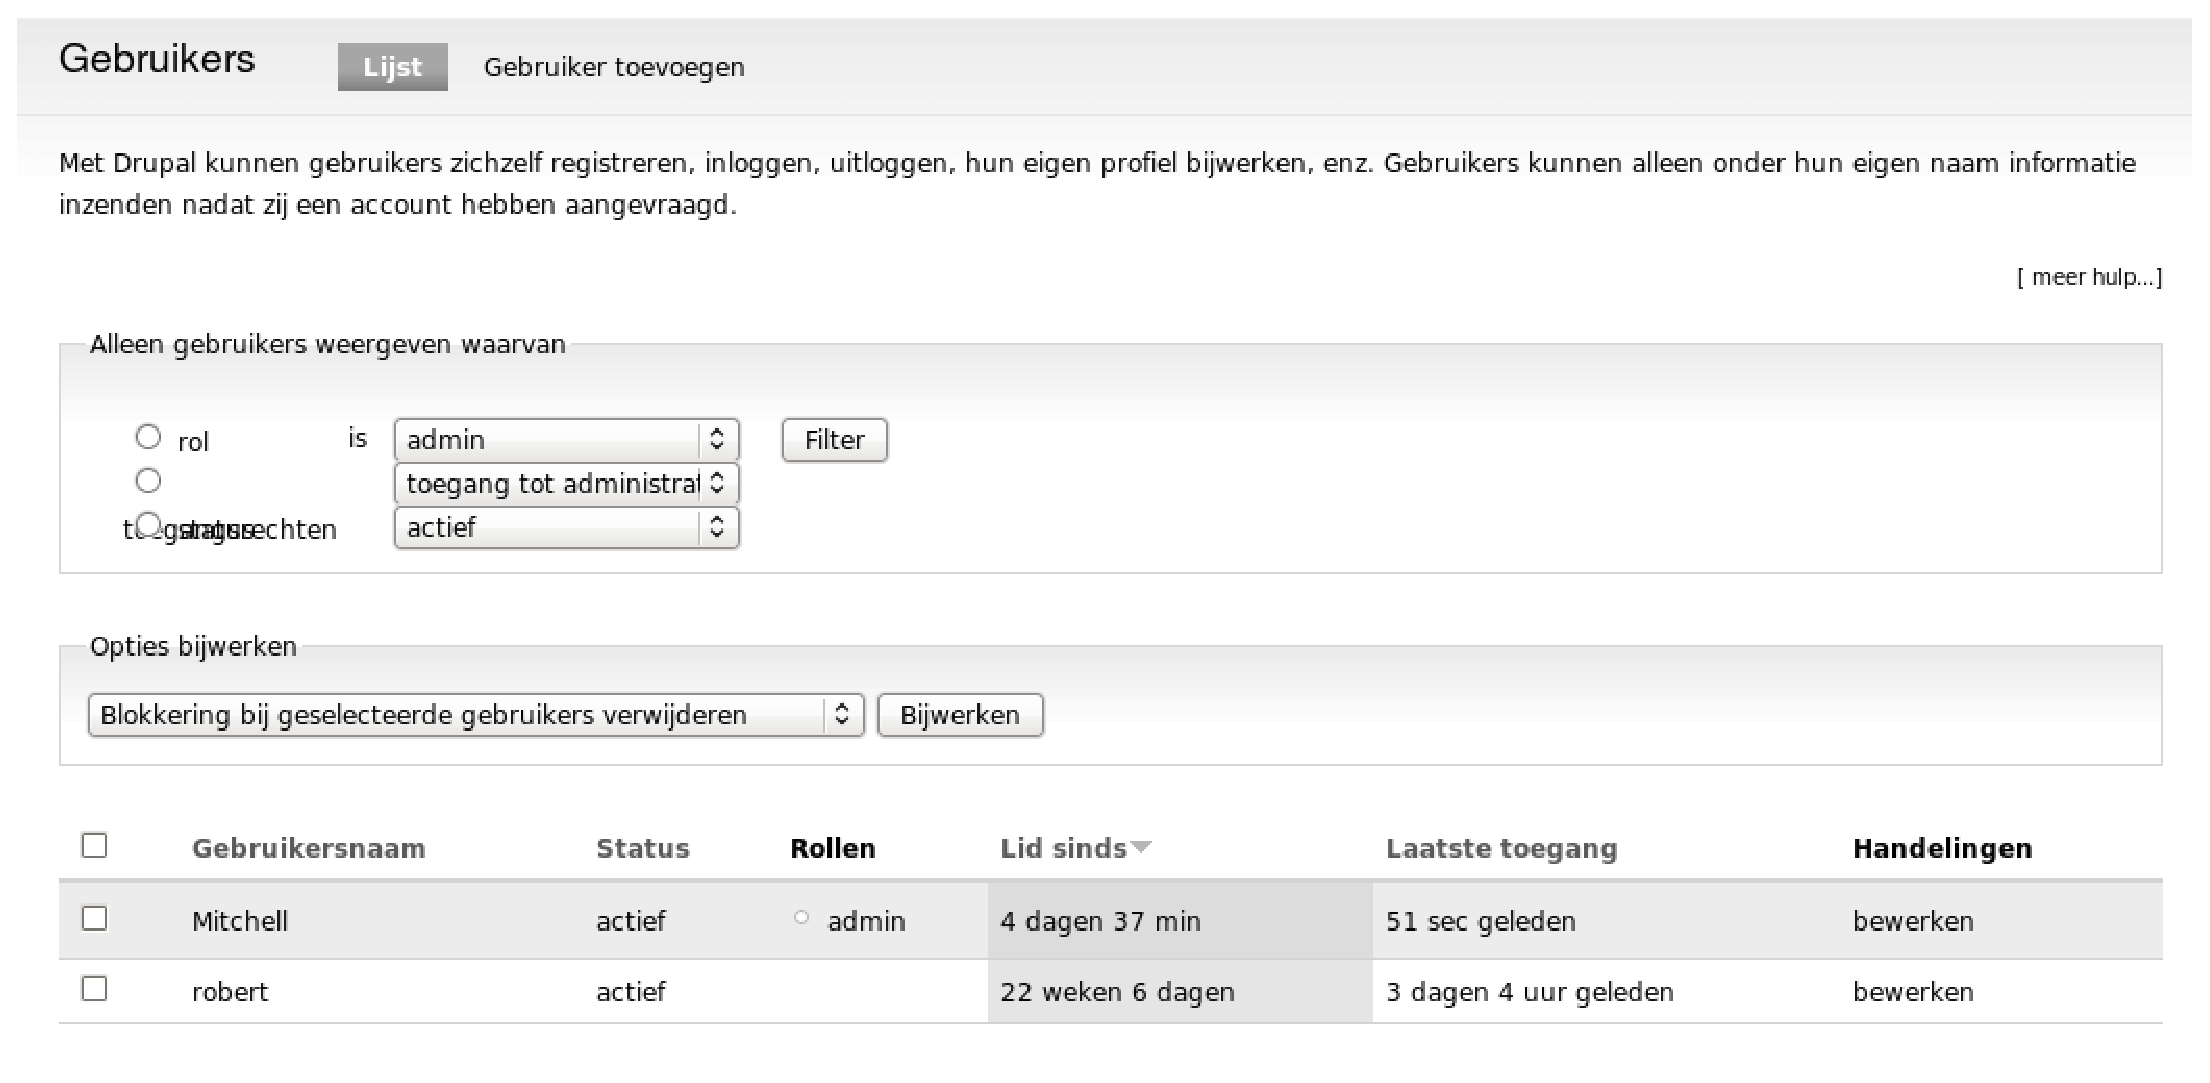
\includegraphics[scale=0.3,angle=0]{gebruikers}
   \caption{gebruikers.\label{white}}
 \end{figure}    
    
\section{Gebruikersinstellingen} \index{gebruikersinstellingen}
    Standaard gedrag voor gebruikers bepalen, waaronder registratievereisten, e-mail en gebruikersafbeeldingen.
\subsection{Instellingen gebruikersregistratie}  \index{gebruikersregistratie}
\begin{figure}[!h]
    \centering
   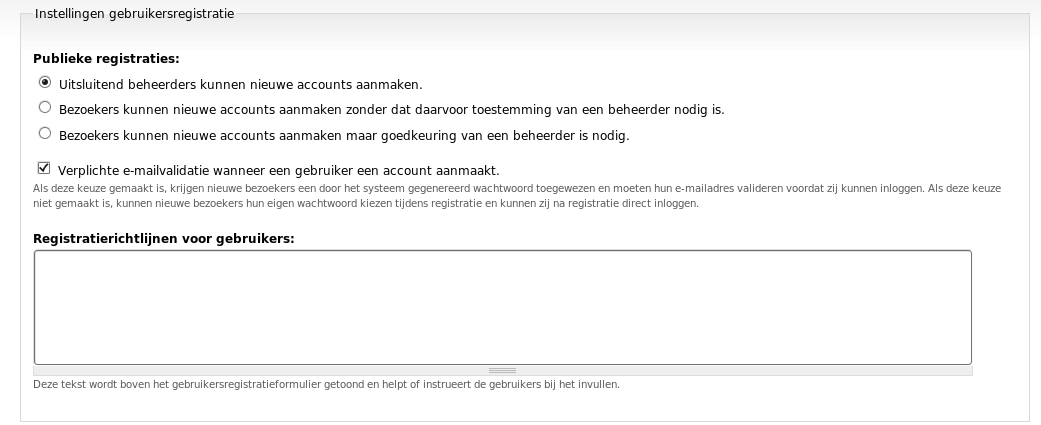
\includegraphics[scale=0.3,angle=0]{publieke-registraties}
   \caption{publieke-registraties.\label{white}}
 \end{figure} 
\subsection{Gebruikersinstellingen e-mail} \index{e-mail}
Drupal stuurt e-mails wanneer een nieuwe gebruiker zich registreert op uw site,
 en optioneel, kan ook gebruikers informeren over andere account-wijzigingen. 
 Gebruikmakend van eenvoudige sjablonen, kunnen informerende e-mails 
 ingesteld worden om te voldoen aan specifieke behoefte van uw site. 
 \begin{figure}[!h]
    \centering
   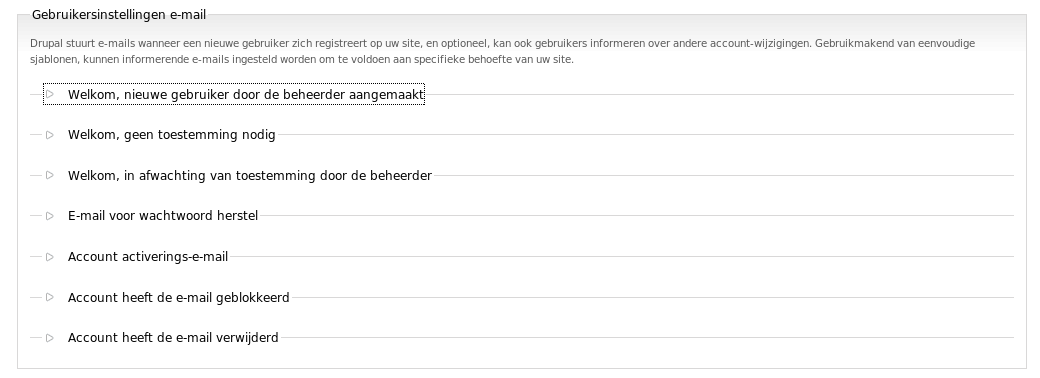
\includegraphics[scale=0.3,angle=0]{gebruikersinstellingen-email}
   \caption{gebruikersinstellingen-email.\label{white}}
 \end{figure} 
    
    
\section{Rollen} \index{rollen}
    Rollen opsommen, toevoegen en wijzigen.
Met rollen kunt u de beveiliging en het beheer van Drupal nauwkeurig bepalen.
 Een rol omvat een groep gebruikers die rechten hebben zoals vastgelegd in toegangsrechten . 
 Voorbeelden van rollen zijn: anonieme gebruiker, geverifieerde gebruiker, moderator, beheerder etc. 
 U kunt zelf de namen van de verschillende rollen bepalen. Met bewerken kunt u een rol verwijderen. 
 Drupal heeft standaard twee rollen:
 \begin{itemize}
\item Anonieme gebruiker: deze rol wordt gebruikt voor gebruikers die geen
account hebben of niet geverifieerd zijn.
\item Geverifieerde gebruiker: deze rol wordt automatisch toegekend aan alle
gebruikers die zijn ingelogd.
\end{itemize}
\begin{figure}[!h]
    \centering
   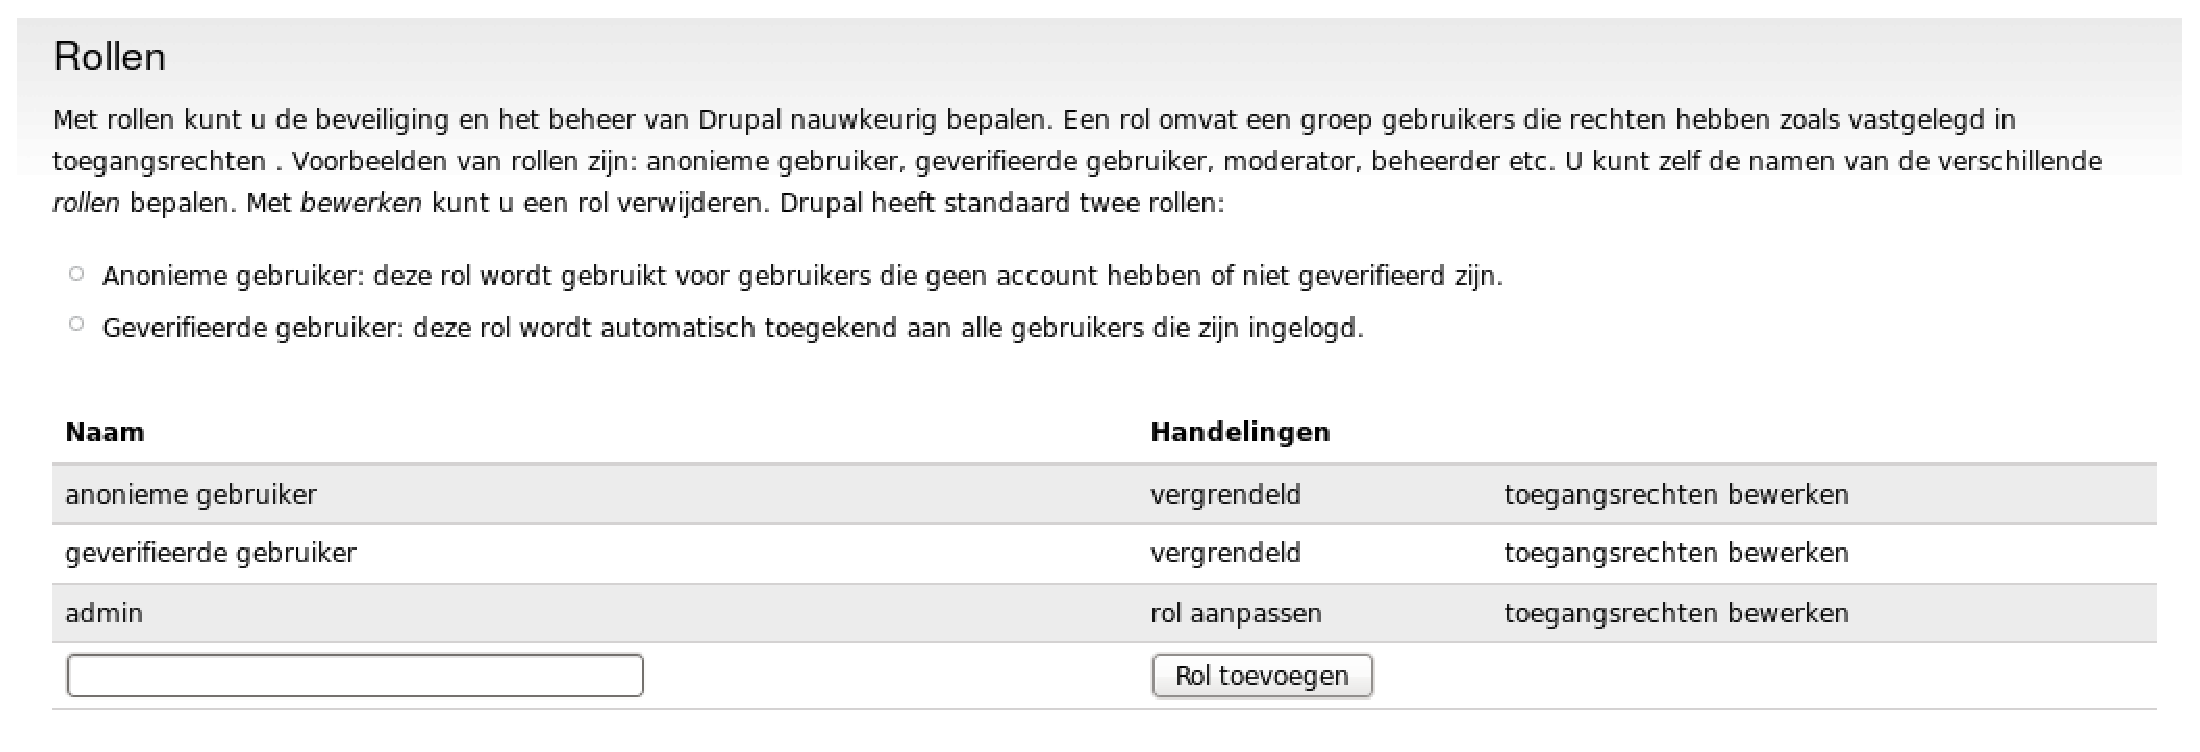
\includegraphics[scale=0.3,angle=0]{rollen}
   \caption{rollen.\label{white}}
 \end{figure} 
 
    
\section{Toegangsrechten} \index{toegangsrechten}
Met toegangsrechten kunt u bepalen wat gebruikers op de site kunnen doen. Iedere
gebruikersrol (gedefinieerd op de pagina rollen) heeft een eigen set toegangsrechten. 
Zo kunt u bijvoorbeeld gebruikers met de rol 'Beheerder' rechten geven voor
'nodes beheren' maar deze mogelijkheid aan gewone 'geverifieerde' gebruikers
onthouden. U kunt de toegangsrechten gebruiken om bepaalde functionaliteit 
beschikbaar te maken voor groepen gebruikers (bijvoorbeeld voor ingelogde gebruikers). 
Met toegangsrechten kan ook de last van het beheren van een drukke site over 
verschillende betrouwbare gebruikers worden verdeeld.
\begin{figure}[!h]
    \centering
   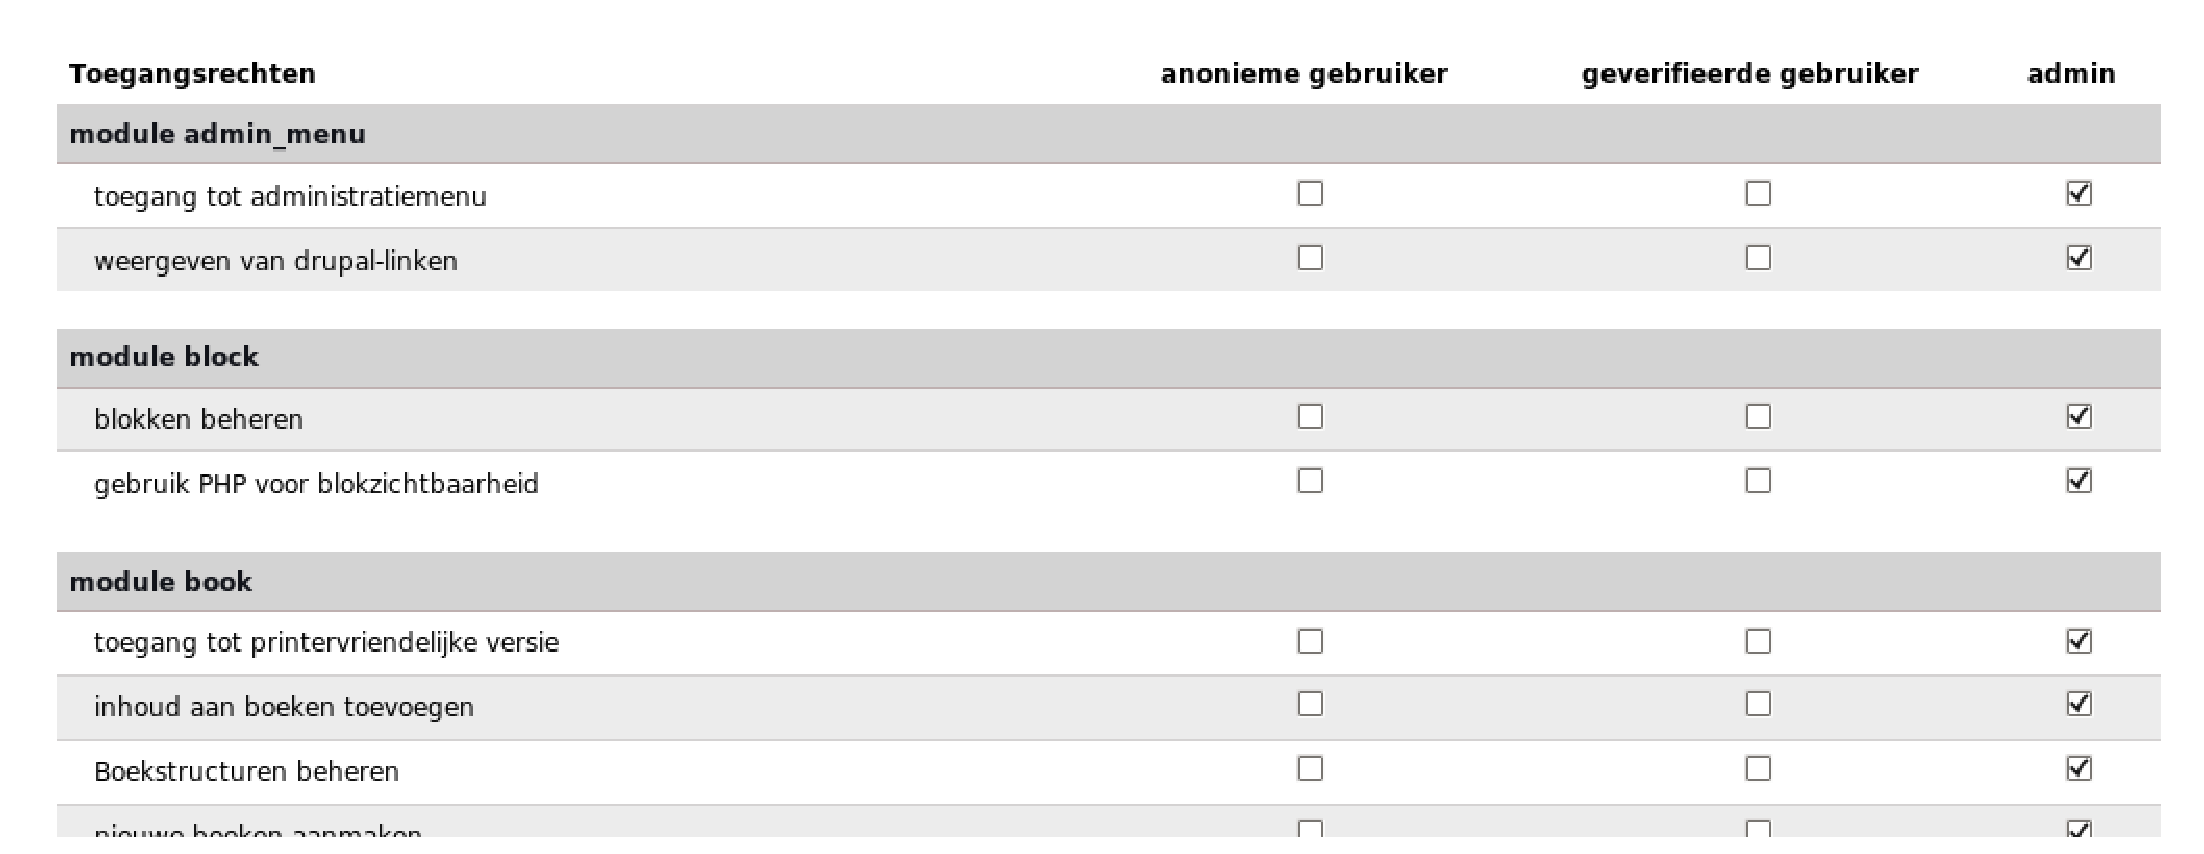
\includegraphics[scale=0.3,angle=0]{toegangsrechten}
   \caption{toegangsrechten.\label{white}}
 \end{figure}


\section{Toegangsregels} 
    Toegangsregels opsommen en aanmaken om gebruikers te weren op basis van gebruikersnaam, e-mailadres en IP-adres.
De toegang op basis van gebruikersnaam en e-mailadres vaststellen voor nieuwe en
bestaande accounts \index{accounts} (account die op dit moment zijn ingelogd
worden niet uitgelogd). Wanneer een gebruikersnaam of e-mailadres overeenkomt met een weigeren-regel en niet met een toestaan-regel, dan zal deze account niet 
mogen inloggen of aangemaakt worden. Een host-regel is werkzaam voor iedere pagina, niet alleen de inlog-pagina.
\begin{figure}[!h]
    \centering
   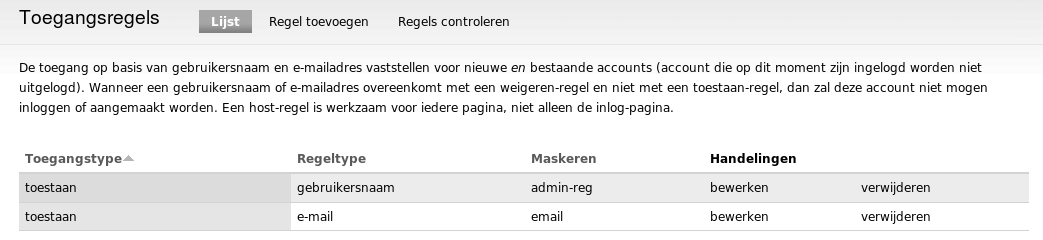
\includegraphics[scale=0.3,angle=0]{toegangsregels}
   \caption{toegangsregels.\label{white}}
 \end{figure}